\documentclass{beamer}
\usepackage{beamerthemesplit}
\usetheme{SPbGU}
%{CambridgeUS}
% Выпишем часть возможных стилей, некоторые из них могут содержать
% дополнительные опции
% Darmstadt, Ilmenau, CambridgeUS, default, Bergen, Madrid, AnnArbor,Pittsburg, Rochester,
% Antiles, Montpellier, Berkley, Berlin
\usepackage{pdfpages}
\usepackage{amsmath}
\usepackage{cmap} % for serchable pdf's
\usepackage[T2A]{fontenc} 
\usepackage[utf8]{inputenc}
\usepackage[english,russian]{babel}
\usepackage{indentfirst}
\usepackage{amsmath}
\usepackage{dot2texi}
\usepackage{tikz}
\usepackage{graphicx}
\usetikzlibrary{shapes,arrows}
% Если у вас есть логотип вашей кафедры, факультета или университета, то
% его можно включить в презентацию.

%\usefoottemplate{\vbox{}}%  \tinycolouredline{structure!25}% {\color{white}\textbf{\insertshortauthor\hfill% \insertshortinstitute}}% \tinycolouredline{structure}% {\color{white}\textbf{\insertshorttitle}\hfill}% }}

%\logo{
\includegraphics[width=1cm]{SPbGU_Logo.png}}

%[GLR-анализатор]
\title[YaccConstructor]{Разработка средств реинжиниринга}
\subtitle[студроект]{Студенческий проект}
\institute[СПбГУ]{
Санкт-Петербургский государственный университет \\
Математико-Механический факультет \\
Кафедра системного программирования }

\lead[Григорьев Семён]{Григорьев Семён Вячеславович}
\date{13 мая 2013г.}

\begin{document}
{
    \begin{frame}
        \begin{center}
            {
\includegraphics[width=1cm]{SPbGU_Logo.png}}
        \end{center}
        \titlepage
    \end{frame}
}

\begin{frame}
	\transwipe[direction=90]
	\frametitle{О проекте}
	\begin{itemize}
		\item Название: YaccConctructor
		\item Сайт проекта: \href{http://recursive-ascent.googlecode.com} {http://recursive-ascent.googlecode.com}
		\item YaccConstructor
		\begin{itemize}
		\item  Модульный инструмент для разработки парсеров и трансляторов для платформы .NET.
		\item Реализован на F\#.
		\item Основная область применения -- реинжиниринг программного обеспечения.
    \end{itemize}
	\end{itemize}
\end{frame}

\author[Рагозина Анастасия]{}

\begin{frame}
	\transwipe[direction=90]
	\frametitle{Задача}
	\begin{itemize}
        \item Разработка парсера (подмножества) языка T-SQL.
        \item Апробация YaccConstructor.
        \item Воспроизвести процесс разработки, характерный для реинжиниринга:
        \begin{itemize}
            \item разработка по доступной документации
            \item цель -- разбор конкретного исходного кода
        \end{itemize}
    \end{itemize}
\end{frame}    

\begin{frame}
	\transwipe[direction=90]
	\frametitle{Особенности реализации}
    \begin{itemize}
        \item В исходной документации присутствуют неточности, которые нужно обрабатывать вручную
        \item Правила из документации нужно переносить по мере необходимости
        \item Для этого важны:
            \begin{itemize}
                \item мощный синтаксис языка спецификации трансляций
                \item алгоритм синтаксического анализа -- GLR
            \end{itemize}
    \end{itemize}
\end{frame}    

\begin{frame}
	\transwipe[direction=90]
	\frametitle{Результаты}
    \begin{itemize}
        \item Рекомендации по доработке YARD/YaccConstructor:
            \begin{itemize}
                \item Дополнительные средства отладки
                \item Необходима полноценная IDE для языка YARD
                \item Нужен контроль качества кода на уровне парсера
                \item light-синтаксис (F\#)
            \end{itemize}
        \item Грамматика подмножества T-SQL
            \begin{itemize}
                \item Основные управляющие конструкции (while, if then else, ...)
                \item DML (Select, update)
                \item Парсер тестировался на 2 млн строк кода. (Уникальных процедур -- 11, 1200 строк кода).
            \end{itemize}
    \end{itemize}
\end{frame}    

\author[Орлов Илья]{}

\begin{frame}
	\transwipe[direction=90]
	\frametitle{Задача}
	\begin{itemize}
        \item Создание библиотеки привязки к исходному коду:
        	\begin{itemize}
                \item Функции сжатия и разжатия тройки координат (id, строка, колонка) и пары координат (id, смещение в файле)
                \item Класс, определяющий биекцию:
                    \begin{itemize}
                        \item между id и именем файла
                        \item между id и картой переносов
	                \end{itemize}
                \item Метод, позволяющий по строке и колонке определить абсолютный отступ (линейное время)
                \item Метод, позволяющий по абсолютному отступу определить строку и колонку (логарифмическое время)
                \item Единицы измерения для данных
            \end{itemize}
        \item Разработка тестов, апробация на парсере T-SQL
    \end{itemize}
\end{frame}    

\begin{frame}
	\transwipe[direction=90]
	\frametitle{Результаты}
	Использование на примере парсера T-SQL
	\begin{itemize}
        \item Cообщение об ошибке: координаты начала и конца
        \item Сокращение объема памяти (за счет сжатия координат):
        \begin{itemize}
            \item Файл: 11 Мб, 300 тыс. строк
            \item Расход оперативной памяти:
            \begin{itemize}
         		\item до сжатия: 665 Мб
          		\item после сжатия: 450 Мб
		    \end{itemize}
            \item Сокращения объема использования оперативной памяти: 32\%
        \end{itemize}
    \end{itemize}
\end{frame}

    
\author[Григорьев Семён]{}

\begin{frame}
	\transwipe[direction=90]
	\frametitle{Результаты}
	\begin{itemize}
        \item Бакаева Алиса. Использование грамматик с весами для автоматической обработки диалектов.
        \item Иванов Андрей. Восстановление после ошибок в GLR-алгоритме.
        \item Алефиров Алексей. Декомпиляция MSIL в F\#.
    \end{itemize}    
\end{frame}

\begin{frame}
	\transwipe[direction=90]
	\frametitle{Результаты}
	\begin{itemize}
        \item В рамках проекта выполняются курсовые работы.
        \item Участники проекта успешно выступили на конференции "Технологии Microsoft в теории и практике программирования 2013"
    \end{itemize}    
\end{frame}

\begin{frame}
	\transwipe[direction=90]
	\frametitle{Демонстрация}
        \begin{center}
            {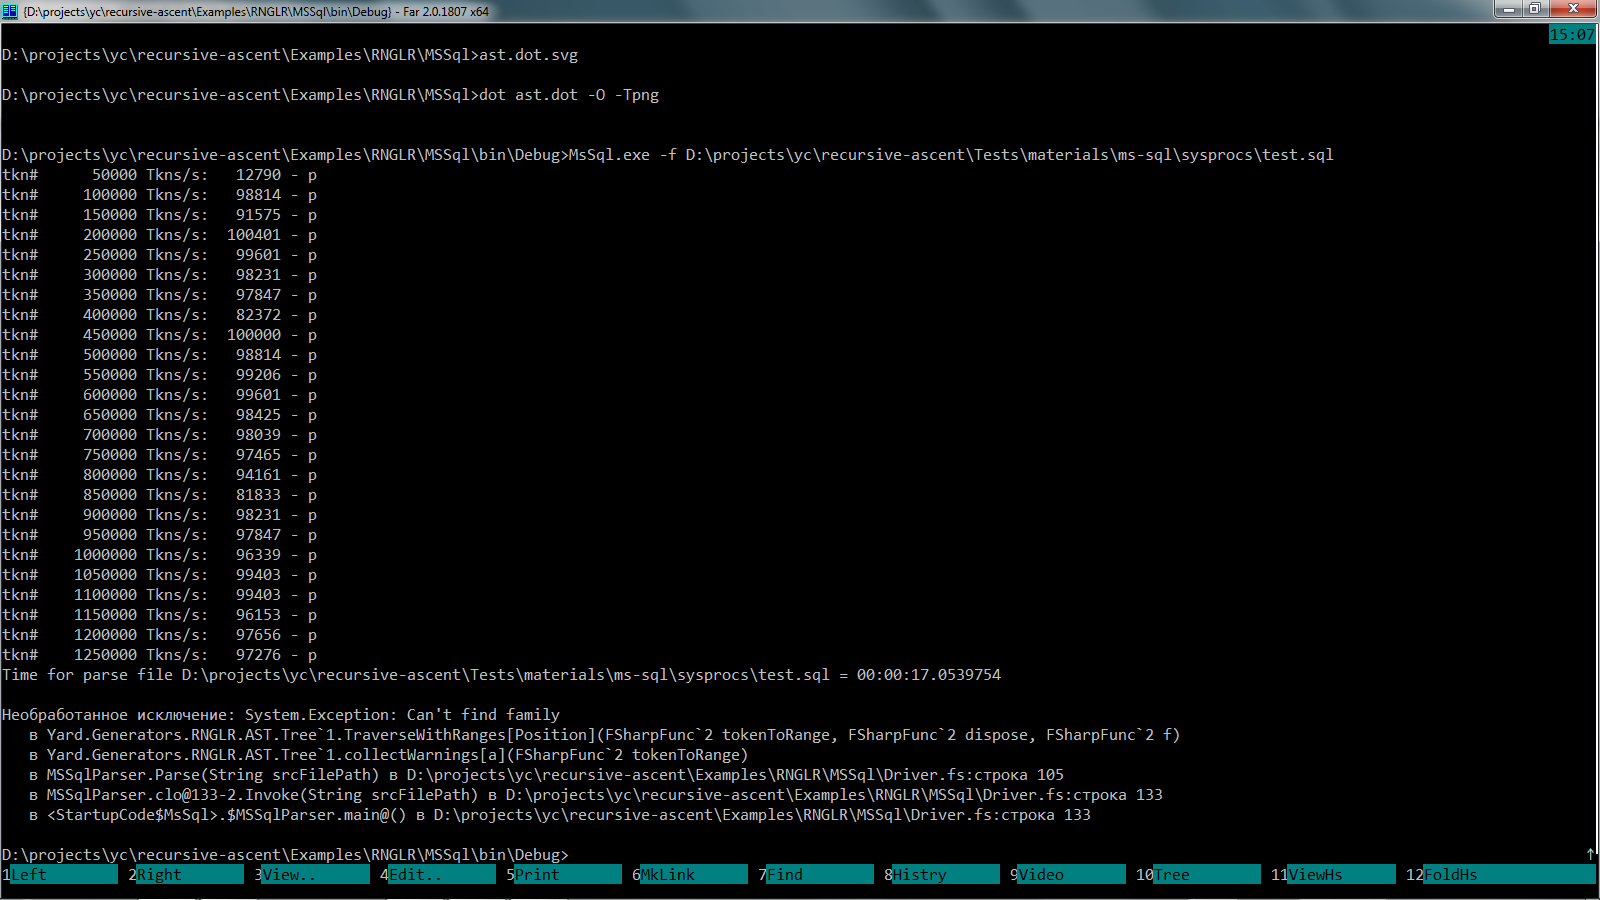
\includegraphics[width=10cm]{demo/demo_picts/p2.png}}
        \end{center}
\end{frame}


\begin{frame}
	\transwipe[direction=90]
	\frametitle{Демонстрация}
        \begin{center}
            {\includegraphics[width=10cm]{demo/demo_picts/ast.pdf}}
        \end{center}
\end{frame}

\begin{frame}
	\transwipe[direction=90]
	\frametitle{Демонстрация}
        \begin{center}
            {\includegraphics[width=10cm]{camel_rev.pdf}}
        \end{center}

\end{frame}



\begin{frame}
	\transwipe[direction=90]
	\frametitle{Заключение}
	\begin{itemize}
        \item Сайт проекта: \href{http://recursive-ascent.googlecode.com} {http://recursive-ascent.googlecode.com}
	    \item Контакты: Semen.Grigorev@lanit-tercom.com
    \end{itemize}    
\end{frame} 

\end{document}
